\chapter{Application Prototype}
\label{ch:Prototype}
Before making a start on of the implementation phase, a lot of effort was put into the creation of the application prototype. Prototyping is a process of developing the initial model of the future application in order to determine the correct application structure, its functionality and the general concept. A prototype is just a model and may differ from the final product.

When designing a new product, the following aspects of the future application should be modelled in order to illustrate the interface concept: the product functionality, relevant user journeys and the visual design. For this purpose, various techniques will be used and the whole modelling process will be described in this chapter. 

First, the project requirements outlined in the previous chapter will be used in order to create a mind map. The map is needed for the initial brainstorming, allowing us to capture and keep together the very raw ideas on the visual side of the project and user experience. In the next step, hand-drawn wireframes will be sketched for every page of the future application. A set of user stories will be created to capture product functionality from the user's perspective. To complement the user stories, a set of scenarios will be developed to describe the user interaction. 

In summary, in this chapter will be described the process of transforming project requirements into the system design. Several design elements (website structure mind map, a set of wireframes) will be produced before the implementation phase. Others (user stories, scenarios and the database schema) will be developed in iterations, alongside with the development of the high level features introduced in the chapter "Requirements Analysis" \ref{ch:requirementanalysis}. During the prototyping phase the focus will be on creating a visually appealling, simple and highly usable design. 

\section{Application Structure}
\label{sec:applicationstructure_prototype}
The prototyping process started with producing a large mind map of the future application. I found mindmapping a very useful way to brainstorm on my ideas, capture and organise them. The final version of the diagram puts together the structure of application pages, navigation scenarios and other ideas relevant to the visual design. A part of the developed mind map can be found in the figure below.

\begin{figure}[H]
	\begin{center}
		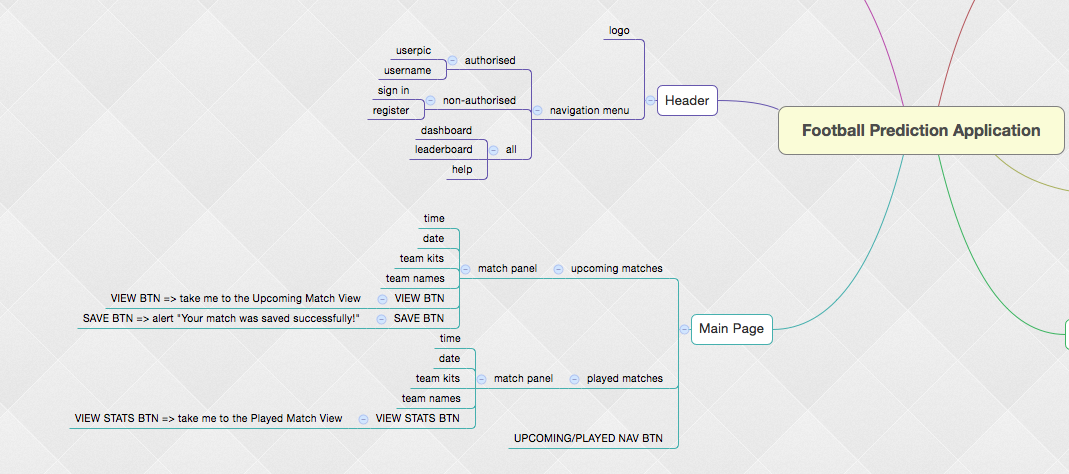
\includegraphics[width=.90\textwidth]{design/images/mindmap}
		\caption{Mind map capturing the results of the initial brainstorming on the application structure and navigation scenarios.}
		\label{fig:using:mindmap}
	\end{center}
\end{figure}

\section{Analysis of the competitors experience}
\label{sec:competitors_prototype}
As the next step, I took another look at the existing websites, expecting to get some ideas on how to approach the visual side of the project and to improve its usability. This step is an important stage of an application prototyping process: it allows to learn from the best design practices and possibly avoid potential errors. The usual practice is to concentrate on few websites of the direct competition as a first step. However, it was not possible to identify the direct competitors, as the idea behind the project is quite unique. Therefore, I analysed several football statistics and community websites, namely \emph{WhoScored?} \citep{source:whoscored}, \emph{Goal.com} \citep{source:goal} and \emph{OLGB Betting Community} \citep{source:olgb}, making a note of how those websites present football statistics to their users, what are the main differences between the presentation of an unplayed and played match, what interesting features each website offer to its audience. This analysis served as a great source of inspiration and the basis for the next step - producing the wireframes.

\section{Wireframes}
\label{sec:wireframes_prototype}
In the early stages of prototyping piece of paper and a pencil are the first choice of many designers. Sketching has a number of advantages when compared to the use of the graphic design software, such as Fireworks or Photoshop. With the editors it is easy to get distracted by brushing up unnecessary details too early. On the opposite side, sketches allow to express the ideas quickly and offer a lot of flexibility. It is easy to add notes, make small changes or replace an outdated sketch with a fresh one.

In case of this project, each of the sketches represented a separate “view” of the website. The scale of a “view” might differ. For example, some sketches show a whole page (home page, dashboard page, etc.), others only capture an important part of a page (a header, a footer, user dropdown menu) in more detail.  Below can be found scans of the paper wireframes.

Scans of the drawings

\section{Branding and Visual Design}
\label{sec:visdesign_prototype}
At this stage of the prototyping process I started thinking of choosing a suitable name for the future application. Below is the list of some names that were considered at this stage.

\begin{itemize}
	\item Too Close To Call
	\item Sure Thing
	\item Footy Expert
	\item Shortening the Odds
\end{itemize}

\emph{SureThing} was chosen as the project name for being unique, simple and catchy, while expressing the essence of the future application. The name evokes optimistic feelings and is quite suitable for a prediction system that is transparent to its users and will increase their chances to win a bet in the long run. 

As it can be seen from the long list of the mandatory requirements, the project will require a lot of time to be invested in implementing its functionality. Therefore, it was decided to make use of the Twitter Bootstrap framework on the front end \citep{documentation:Bootstrap3} \citep{web:templateProgressus} in order to reduce the amount of time spent developing the visual side of the application and create simple and consistent interface. As a result, the final design is a mixture of ready-made solutions and my own ideas on how to visualize unique elements of the application layout, such as dashboard side menu, match panels in matches overview, layout containing prediction modules in upcoming match view, etc. 

\section{User Stories}
\label{userstories_prototype}
User stories serve the same purpose as the more traditional use cases. User sScenarios are a detailed description of how a user will interact with the system. 

concentrate on the use cases - the graphical illustration of the system functionality. UML will be used to design in a clear and readable manner. 

As a User I would like to view the most popular blu-ray discs sold


\begin{figure}[H]
	\begin{center}
		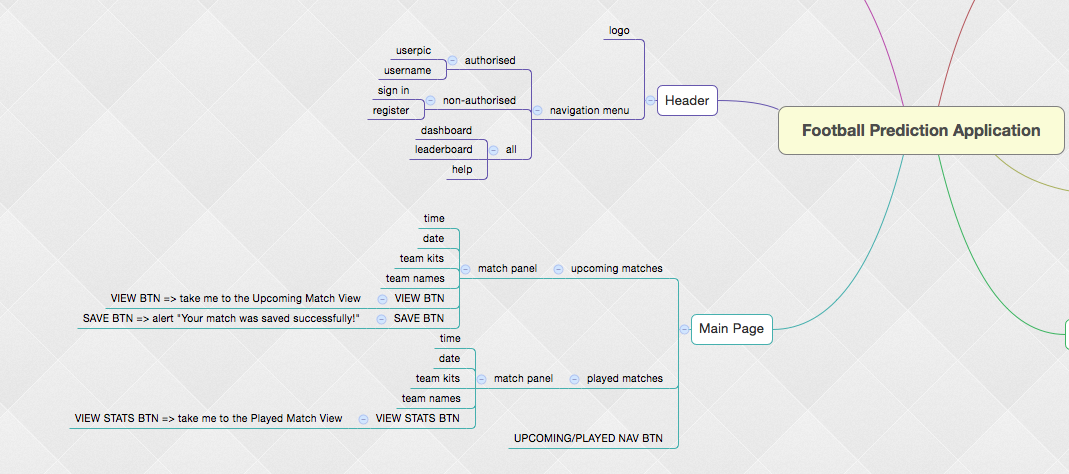
\includegraphics[width=.90\textwidth]{design/images/mindmap}
		\caption{This use case diagram shows the typical sequence of steps a user will take when saving a match to the dashboard.} \label{fig:using:usecase1}
	\end{center}
\end{figure}
This Diagram shows the typical activities a user will complete when using the shared expense area of the application, and how the activities the system will need to complete as a result of some user actions

\section{Database Schema}
\label{databaseschema_prototype}
The application requires a database. The data to be stored in the database will be represented by a set of database models. The database schema for this project was developed in an iterative way along with the development of the high level features of the application: the tables and relationships between them were added gradually. The final, merged version of the diagram is a result of numerous iteration and can be found below.

\begin{figure}[H]
	\begin{center}
		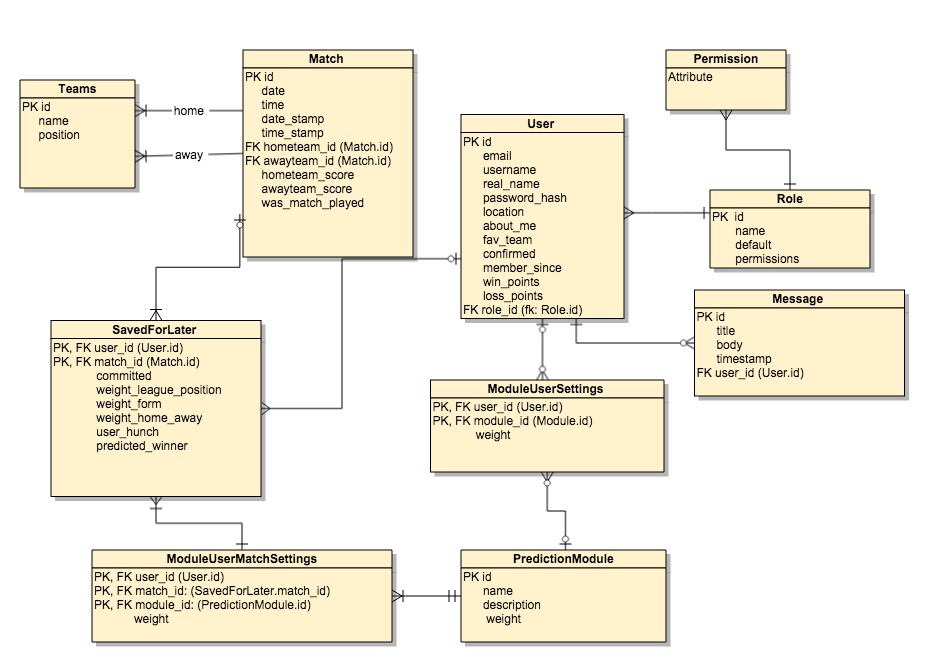
\includegraphics[width=.90\textwidth]{design/images/database_export.jpg}
		\caption{A final diagram representing tables in the database.}
		\label{fig:using:mindmap}
	\end{center}
\end{figure}